\documentclass{ximera}
\input{../preamble}
\addPrintStyle{..}
\begin{document}
	\author{Wiskunde Op Maat}
	\xmtitle{Kwadratische vergelijkingen oplossen}{}

Met deze pagina kan je het oplossen van tweedegraadsvergelijkingen in één onbekende met voorschrift \(ax2+bx+c=0\) inoefenen. 
Onder 'download' kan je de pdf met of zonder antwoorden downloaden.

\newcommand{\choicetwee}{{\wordChoice{\choice[correct]{twee}\choice{één}\choice{geen}}}}
\newcommand{\choiceeen}{{\wordChoice{\choice{twee}\choice[correct]{één}\choice{geen}}}}
\newcommand{\choicegeen}{{\wordChoice{\choice{twee}\choice{één}\choice[correct]{geen}}}}

\newcommand{\choicepositief}{{\wordChoice{\choice[correct]{positief}\choice{nul}\choice{negatief}}}}
\newcommand{\choicenul}{{\wordChoice{\choice{positief}\choice[correct]{nul}\choice{negatief}}}}
\newcommand{\choicenegatief}{{\wordChoice{\choice{positief}\choice{nul}\choice[correct]{negatief}}}}
 
% positieve discriminant 
\begin{exercise}

Bepaal de oplossingen van de vierkantsvergelijking \(x^2 - 4x + 3 = 0\).   

\begin{question}
De discrimant is \choicepositief. 

\begin{feedback}
    Het algemene voorschrift van een tweede graadsvergelijking wordt gegeven door  \(ax^2 + bx + c = 0\). 
    Om een tweedegraadsvergelijking op te lossen bereken je eerst de discriminant \(\Delta = b^2 - 4ac\). 
    Het aantal oplossingen wordt bepaald door het teken van deze discriminant. 
    
\end{feedback}
\end{question}

\begin{question}
    Deze vergelijking heeft \choicetwee oplossingen in de reële getallen. 
    \begin{feedback}
        Indien de discriminant \(\Delta = b^2 - 4ac\) positief is, zijn er twee oplossingen in de reële getallen. 
    \end{feedback}
\end{question}

\begin{question}
    Bepaal de wortels. 
    
    \begin{hint}
        
        Voor een tweedegraadsvergelijking  \(ax^2 - bx + c = 0\) waarbij de discriminant \( \Delta = b^2 - 4ac \) positief is hebben we altijd twee oplossing gegeven door: 
        
        \[
            x_{1} = \frac{-b + \sqrt{\Delta}}{2a}  \text{ en }  x_{2} = \frac{-b - \sqrt{\Delta}}{2a}
            \]
            
            Waarbij:
            \begin{itemize}
                \item \( a \) de coëfficiënt van \( x^2 \) is,
                \item \( b \) de coëfficiënt van \( x \) is,
                \item \( c \) de constante term is,
            \end{itemize}
            
    \end{hint}
    

\end{question}

\begin{oplossing}
            
In het algemeen wordt een tweedegraadsvergelijking in één onbekende gegeven door het voorschrift \(ax^2 - bx + c = 0\). 
De tweedegraadsvergelijking \(x^2 - 4x + 3 = 0\) heeft als coëfficiënten gelijk aan \(a = 1, b = -4 \text{ en } c = 3\). 
We zoeken de getalwaarden voor \(x\) waarvoor deze vergelijking gelijk is aan nul. 
Hiervoor kan de formule met discrimant gebruikt worden. 

\vspace{5mm}

De discrimant \( \Delta = b^2 - 4ac \) is gelijk aan \(\Delta = (-4)^2 -4\cdot 1 \cdot 3\). De vierkanswortel wordt dan gegeven door \(\sqrt{\Delta} = \sqrt{4} = 2\). Er zijn dus twee oplossingen omdat de discriminant positief is. Deze oplossingen worden gegeven door: 

\[
x_{1} = \frac{-b + \sqrt{\Delta}}{2a}  \text{ en }  x_{2} = \frac{-b - \sqrt{\Delta}}{2a}
\]

Invullen levert: 

\[
x_{1} = \frac{-(-4) + \sqrt{4}}{2\cdot 1}  = 3 
\]


\[
x_{2} = \frac{-(-4) - \sqrt{4}}{2\cdot 1}  = 1
\]
 

Als je de vergelijking beschouwd als een functievoorschrift, zijn deze oplossingen de snijpunten van de parabool \( f(x) = x^2 - 4x + 3 \) met de x-as. Aangezien de discriminant positief is, zal de parabool de x-as 2 keer snijden. 

\begin{image}
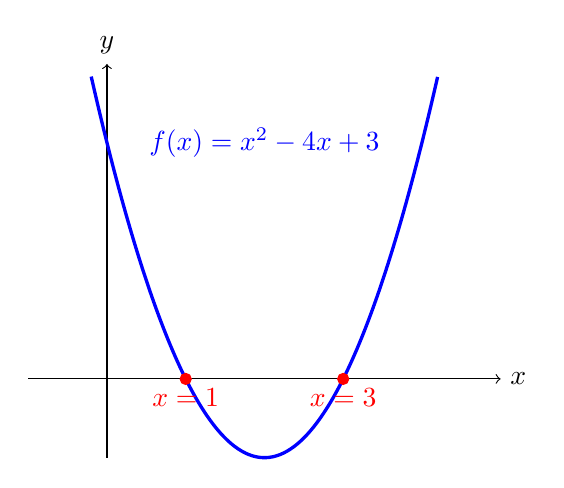
\begin{tikzpicture}[scale=1]

    % Draw axes
    \draw[->] (-1,0) -- (5,0) node[right] {\(x\)};
    \draw[->] (0,-1) -- (0,4) node[above] {\(y\)};
    
    % Draw the parabola y = x^2 - 4x + 3
    \draw[domain=-0.2:4.2, samples=100, smooth, very thick, blue] 
        plot (\x, {(\x)^2 - 4*(\x) + 3}); 
        
    \draw (2, 3) node[blue] {\( f(x) = x^2 - 4x + 3 \)};

    % Roots (zeros) of the parabola
    \filldraw[red] (1,0) circle (2pt) node[below] {\(x=1\)};
    \filldraw[red] (3,0) circle (2pt) node[below] {\(x=3\)};

\end{tikzpicture}
\end{image}

Met de discrimantformule bereken je dus deze snijpunten met de x-as zonder grafiek van de functie . 
\end{oplossing}
  
    
\end{exercise}


% nul discriminant 
\begin{exercise}

    Bepaal de oplossingen van de vierkantsvergelijking \( x^2 - 4x + 4 = 0 \) .

    
    \begin{question}
    De discriminant is \choicenul. 
    \begin{feedback}
        Het algemene voorschrift van een tweede graadsvergelijking wordt gegeven door  \(ax^2 + bx + c = 0\). 
        Om een tweedegraadsvergelijking op te lossen bereken je eerst de discriminant \(\Delta = b^2 - 4ac\). 
        Het aantal oplossingen wordt bepaald door het teken van deze discriminant. 
    \end{feedback}
    \end{question}
    
    \begin{question}
    Deze vergelijking heeft \choiceeen oplossing in de reële getallen. De discrimant is negatief. 
    \begin{feedback}
        Omdat de discriminant nul is hebben we een dubbel nulpunt. 
    \end{feedback}
    \end{question}
    
    \begin{question}
    Bepaal de wortel.
    \begin{hint}
        Voor een tweedegraadsvergelijking \(ax^2 - bx + c = 0\) met \(\Delta = 0\) geldt:
        \[
        x = \frac{-b}{2a}.
        \]
    \end{hint}
    \end{question}
    
    \begin{oplossing}
    In het algemeen wordt een tweedegraadsvergelijking gegeven door het voorschrift \( ax^2 - bx + c = 0 \) 
    Voor de vergelijking 
    \[
    x^2 - 4x + 4 = 0
    \]
    hebben we:
    \[
    a = 1,\quad b = -4,\quad c = 4.
    \]
    
    \vspace{3mm}
    
    Bereken de discriminant:
    \[
    \Delta = b^2 - 4ac = (-4)^2 - 4\cdot1\cdot4 = 16 - 16 = 0.
    \]
    
    Aangezien \(\Delta = 0\) is er één oplossing (dubbele wortel), gegeven door:
    \[
    x = \frac{-b}{2a} = \frac{-(-4)}{2\cdot1} = \frac{4}{2} = 2.
    \]
    
    \vspace{3mm}
    
    Als functievoorschrift is 
    \[
    f(x)=x^2 - 4x + 4
    \]
    een parabool die de x-as raakt in het punt \( (2,0) \).
    
    \begin{image}
    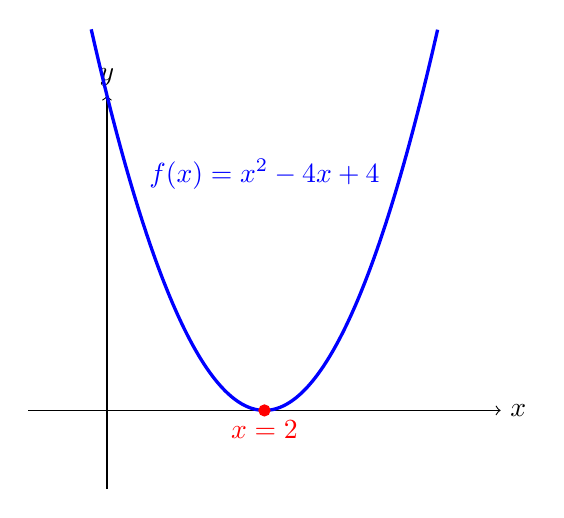
\begin{tikzpicture}[scale=1]
        % Teken de assen
        \draw[->] (-1,0) -- (5,0) node[right] {\(x\)};
        \draw[->] (0,-1) -- (0,4) node[above] {\(y\)};
        
        % Teken de parabool f(x) = x^2 - 4x + 4
        \draw[domain=-0.2:4.2, samples=100, smooth, very thick, blue] 
            plot (\x, {(\x)^2 - 4*(\x) + 4});
            
        \draw (2, 3) node[blue] {\( f(x) = x^2 - 4x + 4 \)};
        
        % Markeer de dubbele wortel
        \filldraw[red] (2,0) circle (2pt) node[below] {\(x=2\)};
        
    \end{tikzpicture}
    \end{image}
    
    \end{oplossing}
      
    
    % \begin{expandable}
    %     \begin{remark}
    %         Aan het functievoorschrift was de dubbele wortel af te lezen als merkwaardig prodcuct aangezien \( f(x) = x^2 - 4x + 4  = (x -2)^2\)
    %     \end{remark}
        
    % \end{expandable}    
    
\end{exercise}


% negatieve disciminant 
\begin{exercise}

    Bepaal de oplossingen van de vierkantsvergelijking \( x^2 - 4x + 5 = 0 \). 
    
    
    \begin{question}
    De discriminant is \choicenegatief.
    \begin{feedback}
        Voor een algemene tweedegraadsvergelijking \(ax^2 - bx + c = 0\) bereken je de discriminant als \(\Delta = b^2 - 4ac\). 
        Hier geldt: 
        \[
        \Delta = (-4)^2 - 4\cdot1\cdot5 = 16 - 20 = -4.
        \]
        Omdat \(\Delta < 0\), is de discriminant negatief.
    \end{feedback}
    \end{question}
    
    \begin{question}
    Deze vergelijking heeft \choicegeen oplossingen in de reële getallen.
    \begin{feedback}
        Wanneer de discriminant negatief is, zijn er oplossingen in de reële getallen. 
        In de algemene formule staat de discriminant onder een wortel. 
        Er is geen reëel getal waarvan het kwadraat negatief is en je kan dus geen oplossingen bepalen: 
        \[
        x_{1} = \frac{-b + \sqrt{\Delta}}{2a}  \text{ en }  x_{2} = \frac{-b - \sqrt{\Delta}}{2a}
        \]

    \end{feedback}
    \end{question}
    
    \begin{oplossing}
    Voor de vergelijking \( x^2 - 4x + 5 = 0 \)
    
    hebben we:
    \[
    a = 1,\quad b = -4,\quad c = 5.
    \]
    
    De discriminant wordt berekend als:
    \[
    \Delta = b^2 - 4ac = (-4)^2 - 4\cdot1\cdot5 = 16 - 20 = -4.
    \]
    
    Aangezien \(\Delta < 0\) zijn er geen reële oplossingen. 

    De grafiek van de parabool ligt volledig boven de x-as. Er zijn geen snijpunten. 
    \begin{image}
        \begin{tikzpicture}[scale=1]
            % Teken de assen
            \draw[->] (-1,0) -- (5,0) node[right] {\(x\)};
            \draw[->] (0,-1) -- (0,6) node[above] {\(y\)};
            
            % Teken de parabool f(x) = x^2 - 4x + 5
            \draw[domain=-0.2:4.2, samples=100, smooth, very thick, blue] 
                plot (\x, {(\x)^2 - 4*(\x) + 5});
                
            \draw (2, 5) node[blue] {\( f(x) = x^2 - 4x + 5 \)};
            
        \end{tikzpicture}
    \end{image}

    
    \end{oplossing}
    
\end{exercise}
    

% \begin{expandable}{remark}{De constante factor \(c\)}
% \begin{remark}
    
    
%     In het algemeen voorschrift \( ax^2+bx+c=0 \) geeft de constante term \(c\) een verticale verschuiving weer. 
%     De waarde van \(c\) heeft dus invloed op het aantal snijpunten met de x-as en hiermee kan je inzien waar die \(c\) ook invloed heeft op het tegen van de discriminant \(\Delta = b^2 - 4ac\). 

% \usepackage{tikz}

%     \begin{image}

%         \begin{scope}[xshift=0cm]
%         \begin{tikzpicture}[scale=1]

%             % Draw axes
%             \draw[->] (-1,0) -- (5,0) node[right] {\(x\)};
%             \draw[->] (0,-1) -- (0,4) node[above] {\(y\)};
            
%             % Draw the parabola y = x^2 - 4x + 3
%             \draw[domain=-0.2:4.2, samples=100, smooth, very thick, blue] 
%                 plot (\x, {(\x)^2 - 4*(\x) + 3}); 
                
%             \draw (2, 3) node[blue] {\( f(x) = x^2 - 4x + 3 \)};
        
%             % Roots (zeros) of the parabola
%             \filldraw[red] (1,0) circle (2pt) node[below] {\(x=1\)};
%             \filldraw[red] (3,0) circle (2pt) node[below] {\(x=3\)};
        
%         \end{tikzpicture}
%         \end{scope}

%         \begin{scope}[xshift=3cm]
%         \begin{tikzpicture}[scale=1]
%             % Teken de assen
%             \draw[->] (-1,0) -- (5,0) node[right] {\(x\)};
%             \draw[->] (0,-1) -- (0,4) node[above] {\(y\)};
            
%             % Teken de parabool f(x) = x^2 - 4x + 4
%             \draw[domain=-0.2:4.2, samples=100, smooth, very thick, blue] 
%                 plot (\x, {(\x)^2 - 4*(\x) + 4});
                
%             \draw (2, 3) node[blue] {\( f(x) = x^2 - 4x + 4 \)};
            
%             % Markeer de dubbele wortel
%             \filldraw[red] (2,0) circle (2pt) node[below] {\(x=2\)};
            
%         \end{tikzpicture}
%         \end{scope}


%         \begin{scope}[xshift=6cm]    
%         \begin{tikzpicture}[scale=1]
%             % Teken de assen
%             \draw[->] (-1,0) -- (5,0) node[right] {\(x\)};
%             \draw[->] (0,-1) -- (0,6) node[above] {\(y\)};
            
%             % Teken de parabool f(x) = x^2 - 4x + 5
%             \draw[domain=-0.2:4.2, samples=100, smooth, very thick, blue] 
%                 plot (\x, {(\x)^2 - 4*(\x) + 5});
                
%             \draw (2, 5) node[blue] {\( f(x) = x^2 - 4x + 5 \)};
            
%         \end{tikzpicture}
%         \end{scope}
        
%     \end{image}
    
    
%     Voor de geïntresseerd leerlingen: de grafiek boven de x-as met een negatieve discrimant in de vierkantswortel heeft geen oplossingen in de reële getallen. 
%     In de complexe getallen hebben wiskundigen echter wel oplossingen gevonden...

%     \begin{expandable}{youtube}{A very gentle introduction to complex numbers.}
%         \youtube{https://youtu.be/f079K1f2WQk}
%     \end{expandable}   

    
% \end{remark}
% \end{expandable}


\begin{exercise} Bepaal de oplossingen van volgende tweedegraadsvergelijkingen. 
  
    \begin{question} De wortels van \( x^2 - 4x + 3    = 0 \) \begin{uitkomst} Er zijn twee reële oplossingen \( 1 \) en  \( 3 \)          \end{uitkomst}\end{question}
    \begin{question} De wortels van \( -2x^2 + 4x + 8  = 0 \) \begin{uitkomst} Er zijn twee reële oplossingen \( -2 \) en  \(4 \)          \end{uitkomst}\end{question}
    \begin{question} De wortels van \( 2x^2 - 8x + 16  = 0 \) \begin{uitkomst} De dubbele wortel is gelijk aan \( 2 \)                     \end{uitkomst}\end{question}
    \begin{question} De wortels van \( 2x^2 + 5x + 2   = 0 \) \begin{uitkomst} Er zijn twee reële oplossingen \( -\frac{1}{2}\) en \(-2 \) \end{uitkomst}\end{question}
    \begin{question} De wortels van \( 3x^2 - 6x + 3   = 0 \) \begin{uitkomst} De dubbele wortel is gelijk aan \( 1   \)                   \end{uitkomst}\end{question}

\end{exercise}


\begin{exercise} Bepaal de oplossingen van volgende tweedegraadsvergelijkingen. 
    
    \begin{question} \( x^2 + 4x + 5    = 0 \) \begin{uitkomst} Er zijn geen oplossingen in de reële getallen.                \end{uitkomst} \end{question}
    \begin{question} \( x^2 + 2x - 8    = 0 \) \begin{uitkomst} Er zijn twee reële oplossingen  \( -4 \) en \( 2 \)           \end{uitkomst} \end{question}
    \begin{question} \( 4x^2 + 12x + 9  = 0 \) \begin{uitkomst} De dubbele wortel is gelijk aan \( -\frac{3}{2} \)            \end{uitkomst} \end{question}
    \begin{question} \( 3x^2 + 6x + 3   = 0 \) \begin{uitkomst} De dubbele wortel is gelijk aan \(  -1 \)                     \end{uitkomst} \end{question}
    \begin{question} \( -x^2 + 4x + 1   = 0 \) \begin{uitkomst} Er zijn twee reële oplossingen  \( -\frac{1}{2} \) en \( 5 \) \end{uitkomst} \end{question}
    
\end{exercise}



\end{document}
